%% @Author: Ines Abdeljaoued Tej
%  @Date:   2018-02
%% @Class:  Posters pour l'ESSAI - Universite de Carthage, Tunisie.

%%%%%%%%%%%%%%%%%%%%%%%%%%%%%%%%%%%%%%%%%
% a0poster Portrait Poster
% LaTeX Template
% Version 1.0 (22/06/13)
%
% The a0poster class was created by:
% Gerlinde Kettl and Matthias Weiser (tex@kettl.de)
%
% This template has been downloaded from:
% http://www.LaTeXTemplates.com
%
% License:
% CC BY-NC-SA 3.0 (http://creativecommons.org/licenses/by-nc-sa/3.0/)
%
%%%%%%%%%%%%%%%%%%%%%%%%%%%%%%%%%%%%%%%%%

%----------------------------------------------------------------------------------------
%	PACKAGES AND OTHER DOCUMENT CONFIGURATIONS
%----------------------------------------------------------------------------------------

\documentclass[a0, portrait]{a0poster}
\usepackage[top=5cm, bottom=0.3cm, left=5cm, right=3cm]{geometry}
\usepackage[compact]{titlesec}
\usepackage{multicol}

\usepackage[frenchb]{babel}
\usepackage{ifxetex}
\ifxetex
  \usepackage{fontspec}
\else
  \usepackage[T1]{fontenc}
  \usepackage[utf8]{inputenc}
  \usepackage{lmodern}
\fi


\usepackage{multicol} % This is so we can have multiple columns of text side-by-side
\columnsep=100pt % This is the amount of white space between the columns in the poster
\columnseprule=3pt % This is the thickness of the black line between the columns in the poster

\usepackage[svgnames]{xcolor} % Specify colors by their 'svgnames', for a full list of all colors available see here: http://www.latextemplates.com/svgnames-colors

\usepackage{times} % Use the times font
%\usepackage{palatino} % Uncomment to use the Palatino font

\usepackage{graphicx} % Required for including images
\graphicspath{{figures/}} % Location of the graphics files
\usepackage{booktabs} % Top and bottom rules for table
\usepackage[font=small,labelfont=bf]{caption} % Required for specifying captions to tables and figures
\usepackage{amsfonts, amsmath, amsthm, amssymb} % For math fonts, symbols and environments
\usepackage{wrapfig} % Allows wrapping text around tables and figures

\begin{document}

%----------------------------------------------------------------------------------------
%	POSTER HEADER
%----------------------------------------------------------------------------------------

% The header is divided into two boxes:
% The first is 75% wide and houses the title, subtitle, names, university/organization and contact information
% The second is 25% wide and houses a logo for your university/organization or a photo of you
% The widths of these boxes can be easily edited to accommodate your content as you see fit

\begin{minipage}[b]{0.75\linewidth}
\VeryHuge \color{NavyBlue} \textbf{Les problèmes avec les écoles en l'Afrique} \color{Black}\\[0.5cm]% Title
\Huge\textit{Une étude détailée sur les problèmes dans les écoles de l'Afrique}\\[0.5cm]% Subtitle
\end{minipage}
%
\begin{minipage}[b]{0.25\linewidth}

\includegraphics[width=7cm]{logo-essai.jpg}
\end{minipage}

\begin{minipage}[b]{0.75\linewidth}
\huge \textbf{Hamza BELHADJ AHMED}\\[0.5cm] % Author(s)
\Large Ecole Sup\'erieure de la Statistique et de l'Analyse de l'Information, Université de Carthage, Tunisie\\[0.4cm] % University/organization
\large \texttt{hmzblhdjahmd@gmail.com}\\
\end{minipage}


\vspace{1cm} % A bit of extra whitespace between the header and poster content

%----------------------------------------------------------------------------------------

\begin{multicols}{3} % This is how many columns your poster will be broken into, a portrait poster is generally split into 2 columns

%----------------------------------------------------------------------------------------
%	ABSTRACT
%----------------------------------------------------------------------------------------

\color{Navy} % Navy color for the abstract

\begin{abstract}
On va étudier et analyser les différents problèmes avec les écoles dans les pays de l'Afrique.

Pour cela, on s'intéresse seulement aux problèmes les plus importantes, c'est-à-dire qui effectuent les plus les élèves.
\end{abstract}
%----------------------------------------------------------------------------------------
%	INTRODUCTION
%----------------------------------------------------------------------------------------

\color{Black} % SaddleBrown color for the introduction
\section*{Introduction}
Les pays de l'Afrique, qui sont des pays non développés, possèdent beaucoup des difficultés sur le plan économique, politique, social, etc.\\
Parmi ces difficultés, on a les problèmes avec les écoles.
Et ces problèmes-là ont des comportements différents selon la région d'étude: urbaine (la ville) ou rurale (le village).

%----------------------------------------------------------------------------------------
%	GEOTHERMAL DATA
%----------------------------------------------------------------------------------------
\section*{Description des données}
\subsection*{Les données}
On a {\color{Red} 6} problèmes avec l'école à analyser:

\begin{itemize}
\item L'école est coûteuse
\item Pas des cahiers et des outils
\item L'absence des enseignants
\item Le mauvais enseignement
\item Les classes surchargés
\item Les facilités pauvres
\end{itemize}

Les deux régions d'étude: urbaine et rurale.

\subsection*{Le comportement de problèmes}
\begin{center}\vspace{1cm}
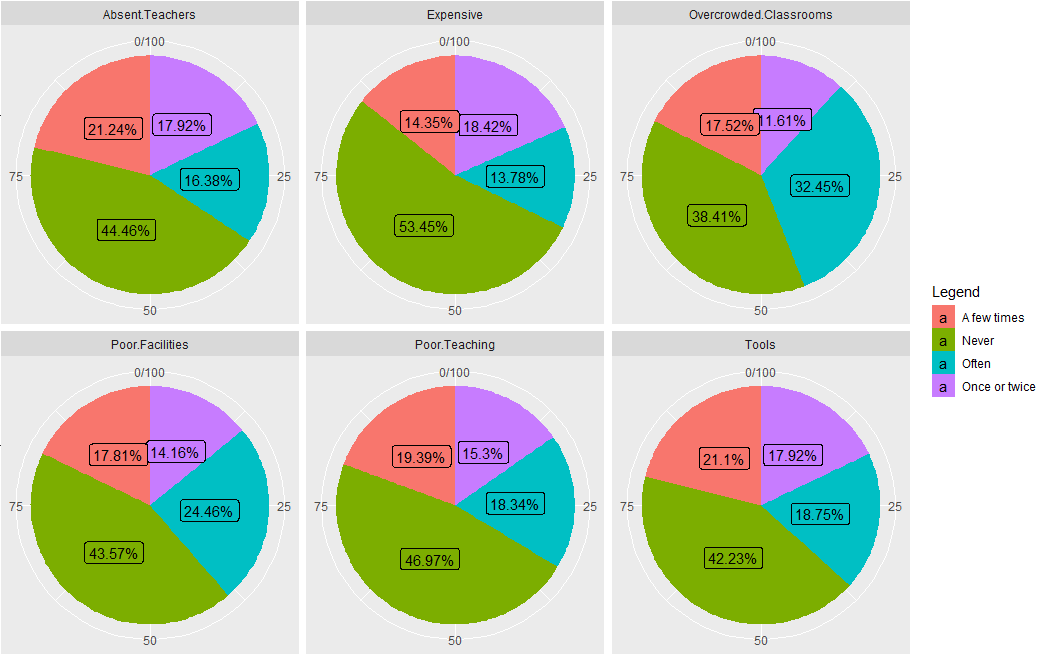
\includegraphics[width=0.8\linewidth]{fig_6_pie.png}
\captionof{figure}{\color{Green} Les six problèmes scolaires par le type de réponse}
\end{center}\vspace{1cm}

On remarque d'abord que la problème des classes surchargés a un taux élevé pour les gens qui répondent 'souvent', ce qui met en valeur l'importance de cette difficulté.

Ensuite, en examinant les problèmes restants, on constante qu'ils sont dépendants et interchangeables, ainsi que les classes surchargés et les facilités pauvres, l'absence des enseignants et le mauvais enseignement, l'école est coûteuse et la mente des cahiers et outils. 

\subsection*{La région et les classes surchargés}
\begin{center}\vspace{1cm}
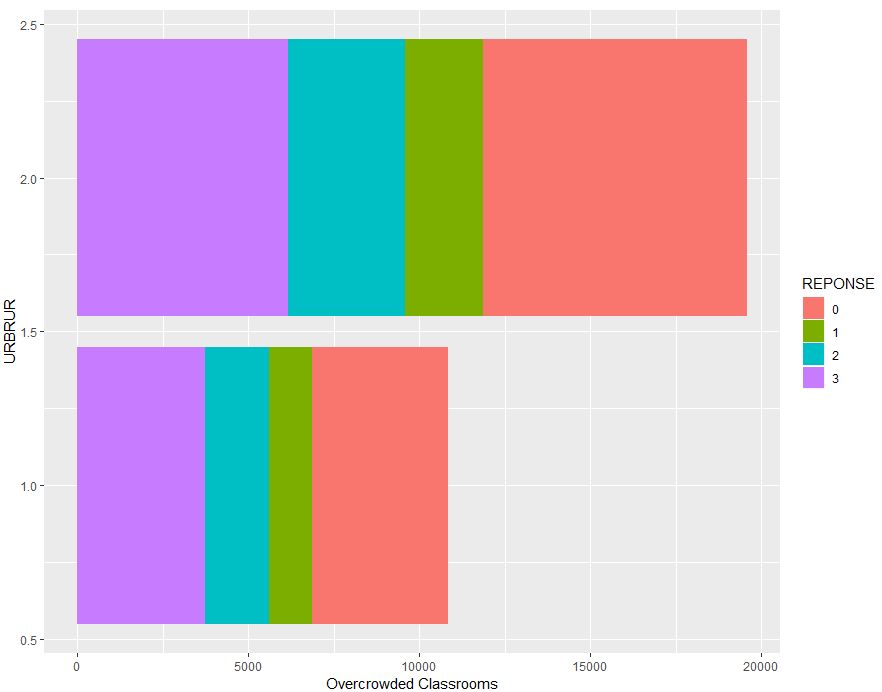
\includegraphics[width=0.8\linewidth]{fig_classrooms_urbrur.png}
\captionof{figure}{\color{Green} Le comportement des classes surchargés selon la région urbaine ou rurale}
\end{center}\vspace{1cm}

En prenant la problème la plus fréquente, c'est-à-dire les classes surchargés, et on l'associer avec la région de question, on constante son importance dans la région rurale par rapport à la région urbaine, c'est que peut être justifier par la pauvreté dans les villages.

%----------------------------------------------------------------------------------------
%	CONCLUSIONS
%----------------------------------------------------------------------------------------

\color{SaddleBrown} % SaddleBrown color for the conclusions to make them stand out

\section*{Conclusions}

On conclure que, dans les pays de l'Afrique, la problème la plus fréquente avec les écoles est les classes surchargés, qui n'est autre qu'une autre problème qui est les facilités pauvres de ces écoles ou la pauvreté en générale de ces pays.
Les autres difficultés ne sont pas moins importantes donc la résolution des telles problèmes est nécessaire pour avoir leur développement.

\color{Black} % Set the color back to DarkSlateGray for the rest of the content

%----------------------------------------------------------------------------------------
%	FORTHCOMING RESEARCH
%----------------------------------------------------------------------------------------

\section*{Perspectives}

Cette étude a nous permis d'avoir une idée comment la pauvreté et la nécessité dans l'Afrique peut effectuer la situation d'écoles.
Notre prochaine étude peut mettre en valeur comment la pauvreté effectue la santé des enfants et des bébés.

%----------------------------------------------------------------------------------------
%	REFERENCES
%----------------------------------------------------------------------------------------

\nocite{*} % Print all references regardless of whether they were cited in the poster or not
\bibliographystyle{plain} % Plain referencing style
\bibliography{sample} % Use the example bibliography file sample.bib
Les données sont extraites de:\\
Afrobarometer Round 5: (https://Afrobarometer.org/fr/data/donnees-fusionnees-de-la-serie-5-34-pays-2015)

%----------------------------------------------------------------------------------------

\end{multicols}
\end{document}